\title{Bras mécanique et sudoku}
\author{Laurent Tainturier \& Alphonse TERRIER}
\date{2016-2017}
\documentclass[12pt,a4paper]{report}
\usepackage[utf8]{inputenc}
\usepackage[T1]{fontenc}
\usepackage[french]{babel}
\usepackage{hyperref}
\usepackage{lmodern}
\usepackage{graphicx}
\usepackage{multirow}
\usepackage{listings}
\usepackage{enumitem}
\usepackage{stmaryrd}
\usepackage{animate}
\usepackage{url}
\usepackage{array}
\usepackage{amsmath, amsfonts, amssymb}
%\usepackage{minted}
\usepackage{color}
\usepackage{tabularx}
\usepackage{float}
\usepackage{caption}
\usepackage[backend=biber, autolang=other, sorting=none, style=science]{biblatex}
\usepackage[left=4cm,right=3cm,top=2.5cm,bottom=2.5cm]{geometry}
\usepackage{fancyvrb}
\frenchbsetup{StandardLists=true}
\newtheorem{theo}{Définition}[section]
\definecolor{lightgray}{gray}{.6}
\usepackage[dvipsnames]{xcolor}
\definecolor{yellow}{RGB}{225,220,0}
\hypersetup{pdfborder={0 0 0}}

\newenvironment{changemargin}[2]{\begin{list}{}{%
\setlength{\topsep}{0pt}%
\setlength{\leftmargin}{0pt}%
\setlength{\rightmargin}{0pt}%
\setlength{\listparindent}{\parindent}%
\setlength{\itemindent}{\parindent}%
\setlength{\parsep}{0pt plus 1pt}%
\addtolength{\leftmargin}{#1}%
\addtolength{\rightmargin}{#2}%
}\item }{\end{list}}

\usepackage{placeins}

%\addbibresource{bibli.bib}

\begin{document}
\FloatBarrier

\begin{titlepage}
\begin{changemargin}{-1cm}{0cm}
	\centering
	\vspace{5cm}
	{\scshape\huge Institut Supérieur d'Électronique de Paris \par}
	\vspace{1cm}
	{\scshape\LARGE TIPE\par}
	\vspace{1.5cm}
	{\fontsize{45}{45}\selectfont\bfseries Bras mécanique et sudoku\par}
	\vspace{2cm}
	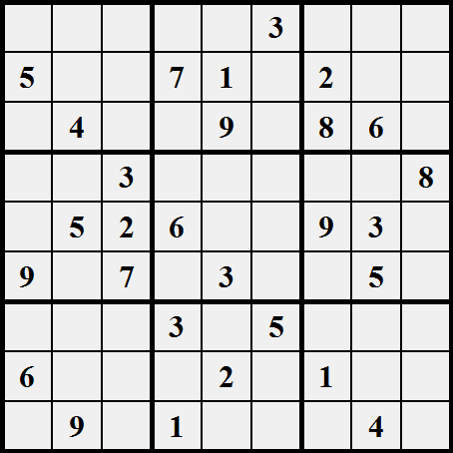
\includegraphics[width=0.7\textwidth]{../pictures/pagedegarde.png}\par\vspace{1.5cm}
	{\LARGE Laurent Tainturier \& Alphonse Terrier\par}
	\vfill
	\large supervisé par\par
	\large \bfseries M. Patrick COUVEZ

	\vfill

	{\large 2016-2017}
\end{changemargin}
\end{titlepage}

\tableofcontents
\addcontentsline{toc}{chapter}{Introduction}
	\chapter*{Introduction}
\footnote{Sauf mention contraire, les images et figures ont été réalisées par nos soins.}
	
	\chapter{Présentation et faits sur le sudoku}
	
	Le sudoku est un jeu sous forme de grille inspiré du carré latin et défini en 1979 par Howard Garns.
	
	Cette grille est carrée et est divisée en $n^2$ régions de $n^2$ cases. Elle possède ainsi $n^2$ colonnes, $n^2$ lignes et $n^4$ cases. Dans la version la plus commune : $n=3$. On appelle section, une ligne, une colonne ou une région

Une grille de sudoku est préremplie, le but du jeu étant de la compléter selon la règle suivante :
\begin{itemize}[label=--]
\item Chaque section doit contenir au moins une fois tous les de $1$ à $n^2$.
\end{itemize} 

Une grille est considérée comme sudoku seulement si sa solution est unique.

Le minimum de cases remplies au préalable pour espérer que la dite solution soit bien unique est de 17, cela a été prouvé par une équipe islandais en 2012.

	\chapter{Mécanique}	
	\section{Choix concernant la structure du bras}
	La premier défi qui s'est imposé à nous a été le choix d'une structure adéquate : solide et pratique. Notre choix s'est alors porté sur les Makerbeam. MakerBeam est un système de construction Open-Source basé sur des profilés ALU en T.
	
	L'écriture se fera en coordonnées polaires et non pas en coordonnées cartésiennes pour les raisons suivantes :
	\begin{itemize}[label=--]
	\item un système en coordonnées cartésiennes aurait été trop encombrant et un moins "portable" (dans un contexte notamment d'optimalité, comme exigé par le programme)
	\item c'est un défi technique de fabriquer un bras de ce type en coordonnées polaires
	\end{itemize}
	
Ainsi, un moteur pas-à-pas assurera la rotation $\theta$ du bras. Ce moteur s'auto-entrainera autour d'une roue dentée de 128 dents comme celle-ci et un roulement permettra la rotation de l'entièreté du bras :

\begin{figure}[!h]
 \center
 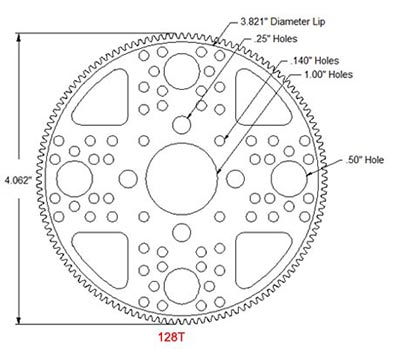
\includegraphics[scale=0.5]{../pictures/rouedentee2.jpg}
 \caption{Schéma de la roue dentée}
\end{figure}


De même la translation $r$ a été assurée par un deuxième moteur pas-à-pas et un système courroie/poulie. Cette translation s'est faite le long de deux axes de $272$ mm et de $8$ mm de diamètre.

	\section{Étude cinématique du mécanisme}
	La pièce 0 correspondra par la suite au bâti. La base du bras et le bâti seront supposés en liaison encastrement, alors qu'ils sont en réalité en liaison appui-plan, cependant les forces de frottements entre ces deux pièces sont telles quelles sont immobiles l'une par rapport à l'autre. La pièce 2 correspond à la structure du bras, reposant sur la roue dentée. La pièce 3 symbolise le chariot et la pièce 3 le stylo.

\begin{figure}[!h]
 \center
 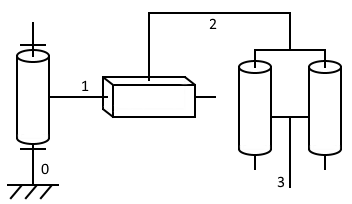
\includegraphics[scale=1.1]{../pictures/schema_cinematique.png}
 \caption{Schéma cinématique du mécanisme choisi}
\end{figure}

	Les deux liaisons en parallèle entre 2 et 3 peuvent être remplacés par une liaison équivalentede torseur $\{ T_c (2/3) \}$ devant vérifier l'équation suivante: : 
	\begin{align*}
\{ T_c (2/3) \}_{B} = \{ T'_c (2/3) \}_{B} = \{ T''_c (2/3) \}_{B}
\end{align*}
On notera les liaisons entre les pièces 2 et 3 $L'_{2/3}$ et $L''_{2/3}$. On a alors:
\begin{align*}
\{ T'_c (2/3) \} =
\begin{array}{c}
	\\ \\ \\ 
\end{array} _{\forall P \in (B,\overrightarrow{z})}
\left\{
\begin{array}{cc}
	0 & 0 \\
	0 & 0 \\
	\gamma'_{2/3} & w'_{2/3} \\
\end{array}
\right\} _{x,y,z)}
\end{align*} 
\begin{align*}
\{ T''_c (2/3) \} = 
\begin{array}{c}
	\\ \\ \\ 
\end{array} _{\forall P \in (C, \overrightarrow{z})}
\left\{
\begin{array}{cc}
	0 & 0 \\
	0 & 0 \\
	\gamma''_{2/3} & w''_{2/3} \\
\end{array}
\right\} _{(x, y, z)}
\end{align*}
\begin{align*}
\mbox{Or } \overrightarrow{V}(B \in 2/3) 
&= \overrightarrow{V}(C \in 2/3)+\overrightarrow{\Omega}(2/3) \wedge \overrightarrow{CB}\\ 
&= w''_{2/3} \overrightarrow{z} + \gamma''_{2/3} \overrightarrow{z} \wedge BC \overrightarrow{x} \\
&= w''_{2/3} \overrightarrow{z} + \gamma''_{2/3}BC \overrightarrow{y}
\end{align*} 
\begin{align*}
\mbox{On a donc }
\{ T''_c (2/3) \} = 
\begin{array}{c}
	\\ \\ \\ 
\end{array} _{B}
\left\{
\begin{array}{cc}
	0 & 0 \\
	0 & \gamma''_{2/3}BC \\
	\gamma''_{2/3} & w''_{2/3} \\
\end{array}
\right\} _{(x, y, z)}
\end{align*}
\begin{align*}
\mbox{Donc }
\{ T_c (2/3) \} = 
\begin{array}{c}
	\\ \\ \\ 
\end{array} _B
\left\{
\begin{array}{cc}
	0 & 0 \\
	0 & 0 \\
	\gamma'_{2/3} & w'_{2/3} \\
\end{array}
\right\} _{x,y,z)} =
\begin{array}{c}
	\\ \\ \\ 
\end{array} _{B}
\left\{
\begin{array}{cc}
	0 & 0 \\
	0 & \gamma''_{2/3}BC \\
	\gamma''_{2/3} & w''_{2/3} \\
\end{array}
\right\} _{(x, y, z)}
\end{align*} 
\begin{align*}
\mbox{D'où le système d'équation : }
\left\{
\begin{array}{l}
0 = 0 \\
0 = 0 \\
\gamma'_{2/3} = \gamma''_{2/3} \\
0 = 0 \\
\gamma''_{2/3} = 0 \\
w'_{2/3} = w''_{2/3} \\
\end{array}
\right. 
\end{align*} 
\begin{align*}
\mbox{On en déduit } 
\{ T_c (2/3) \} = 
\begin{array}{c}
	\\ \\ \\ 
\end{array} _B
\left\{
\begin{array}{cc}
	0 & 0 \\
	0 & 0 \\
	0 & w'_{2/3} \\
\end{array}
\right\} _{x,y,z)}
\end{align*}

La liaison équivalente est donc une liaison glissière d'axe z, ce qui permet des déplacements verticaux du stylo, il peut ainsi être mis en contact avec la feuille.
On a alors le schéma de la figure \ref{Schema_cine_simp}.

\begin{figure}[!h]
 \center
 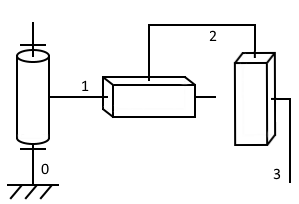
\includegraphics[scale=1.1]{../pictures/schema_cinematique_simplifie.png}
 \caption{Schéma cinématique équivalent du mécanisme choisi}
 \label{Schema_cine_simp}
\end{figure}

	\section{Difficultés rencontrées et solutions mises en place}
	Nous avons notamment rencontré des difficultés concernant le roulement utilisé. En effet, nous avions au préalable utilisé un roulement à billes comme celui-ci :
	
	\begin{figure}[!h]
 \center
 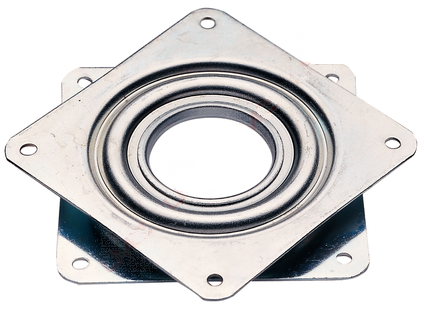
\includegraphics[scale=0.5]{../pictures/roulementmerdique}
 \caption{Roulement défectueux}
\end{figure}

Malheureusement, ce roulement tournait très mal et saccadait. De plus, du jeu était présent. Après quelques heures de recherche, nous avons donc choisi le roulement à billes suivant, qui tourne très bien mais qui tout de même possède lui aussi un peu de jeu :

	\begin{figure}[!h]
 \center
 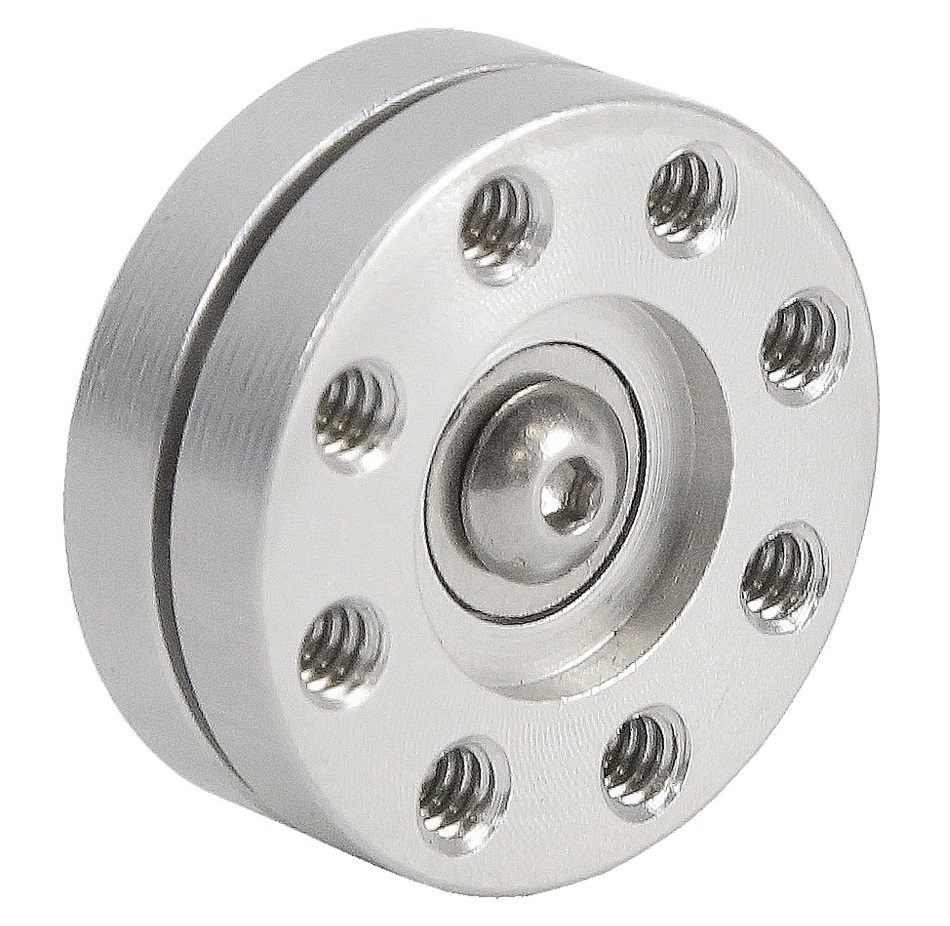
\includegraphics[scale=0.15]{../pictures/swivelhub}
 \caption{Roulement finalement choisi}
\end{figure}

	
	
	\section{Conception du chariot en 3D}
	Nous avons pris la décision de concevoir certaines pièces de notre projet en 3D, celle-ci nécessitant de la précision. Le logiciel professionnel de modélisation SolidWorks, développé par DassaultSystèmes, a été utilisé pour développer ces pièces.
	
	Les mises en plan des pièces composant le chariot sont disponibles en annexe \ref{chariot} à partir de la page \pageref{chariot}.
	
	La partie principale du chariot devait pouvoir accueillir un servomoteur, permettant l'abaissement et le soulèvement du stylo :
	
	%\begin{figure}[!h]
 %\center
 %\includegraphics[scale=0.15]{../pictures/chariot}
 %\caption{Impression 3D de la pièce principale du chariot}
	%\end{figure}
	
	Ce stylo sera fixé sur la pièce présentée en page \pageref{supportstylo} dont l'impression 3D est montrée ci-dessous :
	
	%\begin{figure}[!h]
 %\center
 %\includegraphics[scale=0.15]{../pictures/supportstylo}
 %\caption{Impression 3D de la pièce supportant le stylo}
	%\end{figure}
	
L'ensemble chariot/support du stylo imprimé en 3D est alors montrée ci-dessous :

	%\begin{figure}[!h]
 %\center
 %\includegraphics[scale=0.15]{../pictures/supportchariot}
 %\caption{Impression 3D du chariot et du support du stylo}
	%\end{figure}

Le chariot permet, de façon modulaire, d'accueillir un support caméra se divisant en deux pièces présentées en page \pageref{chariotcamera} et en page \pageref{supportcamera}.
	

	\chapter{Électronique}
\section{Moteurs pas-à-pas}
\label{Elec_stepper}
Nous avons utilisés dans ce projet deux moteurs pas-à-pas qui présentaient, par rapport à d'autres types de moteurs, les avantages suivants : 
\begin{itemize}[label=--,itemsep=0pt,font=\bf\Large,labelsep=5mm]
\item une précision bien supérieure à celle de moteurs à courant continu;
\item un couple bien plus important que celui de servomoteurs;
\item mis sous tension, un déplacement fortuit du moteur n'est pas possible.
\end{itemize}
Les moteurs pas-à-pas sont notamment utilisés dans les systèmes nécessitant une grande précision comme les imprimantes 3D dans lesquelles ils sont très largement employés.

\begin{figure}[!h]
 \center
 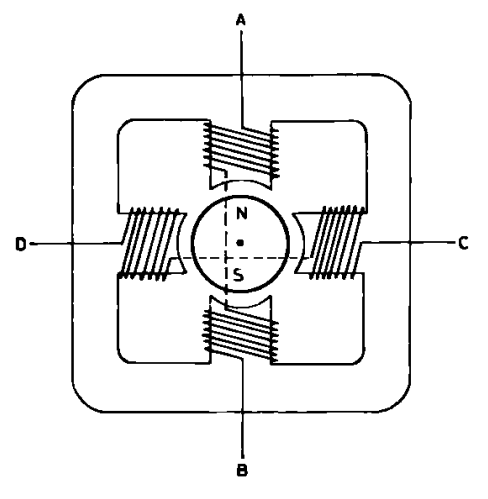
\includegraphics[scale=0.38]{../pictures/schema_stepper_motor.png}
 \caption{Schéma simplifiée d'un moteur pas-à-pas\protect\footnotemark}
 \label{schema_stepper}
\end{figure}
\footnotetext{\url{http://eskimon.fr/290-arduino-603-petits-pas-le-moteur-pas-pas}}

\paragraph{} Les moteurs que nous avons utilisés sont constitués de deux bobines, repliées tout autour de la partie centrale du moteur, permettant des petits déplacements de la partie mobile. Celles-ci sont divisées en deux sur la figure \ref{schema_stepper}. La bobine 1 a pour extrémités A et B; la bobine 2 C et D. Ces bobines, lorsqu'elles sont parcourues par un courant i, génèrent un champ magnétique. Ce champ magnétique a pour conséquence d'entrainer la rotation de la partie mobile du moteur : le rotor, représenté par le cercle centrale N/S. Celui-ci est composé d'un aimant qui a tendance a s'aligner sur le champ magnétique créé par les bobines. 
Les bobines sont enroulées autour d'un fer doux, généralement de la ferrite afin de mieux conduire le lignes de champs.

\paragraph{} On distingue deux types de fonctionnement pour ces moteurs bipolaires, un fonctionnement à demi-pas et un fonctionnement à pas complet. Nous avons retenu ce dernier système car il permettait d'obtenir une vitesse et un couple constants lors de la rotation des moteurs. 
Comme le montre la figure \ref{Motor_min}, à chaque séquence, une seule bobine suffirait à mettre en mouvement le moteur, cependant nous avons choisi d'alimenter tout de même l'autre afin d'obtenir un couple maximal (cf figure \ref{Motor_max}). 

\begin{center}
\renewcommand{\arraystretch}{1.25}
\begin{tabularx}{0.49\linewidth}{|c|*{5}{>{\centering \arraybackslash}X|}}\hline
\multirow{2}*{Séquence} & \multicolumn{2}{c|}{Bobine 1}  & \multicolumn{2}{c|}{Bobine 2} \\
\cline{2-5} & \centering A & \centering B & \centering C & D \\ \hline  
1 & 1 & 0 & - & - \\ \hline
2 & - & - & 0 & 1 \\ \hline
3 & 0 & 1 & - & - \\ \hline
4 & - & - & 1 & 0 \\ \hline
5 & 1 & 0 & - & - \\ \hline
\end{tabularx}
\captionof{table}{Séquences d'alimentation des bobines avec un couple minimal}
\end{center}

\begin{center}
\renewcommand{\arraystretch}{1.25}
\begin{tabularx}{0.49\linewidth}{|c|*{5}{>{\centering \arraybackslash}X|}}\hline
\multirow{2}*{Séquence} & \multicolumn{2}{c|}{Bobine 1}  & \multicolumn{2}{c|}{Bobine 2} \\
\cline{2-5} & \centering A & \centering B & \centering C & D \\ \hline  
1 & 1 & 0 & 0 & 1 \\ \hline
2 & 0 & 1 & 0 & 1 \\ \hline
3 & 0 & 1 & 1 & 0 \\ \hline
4 & 1 & 0 & 1 & 0 \\ \hline
5 & 1 & 0 & 0 & 1 \\ \hline
\end{tabularx}
\captionof{table}{Séquences d'alimentation des bobines avec un couple maximal}
\end{center}

\begin{center}
\begin{figure}[!h]
 \center
 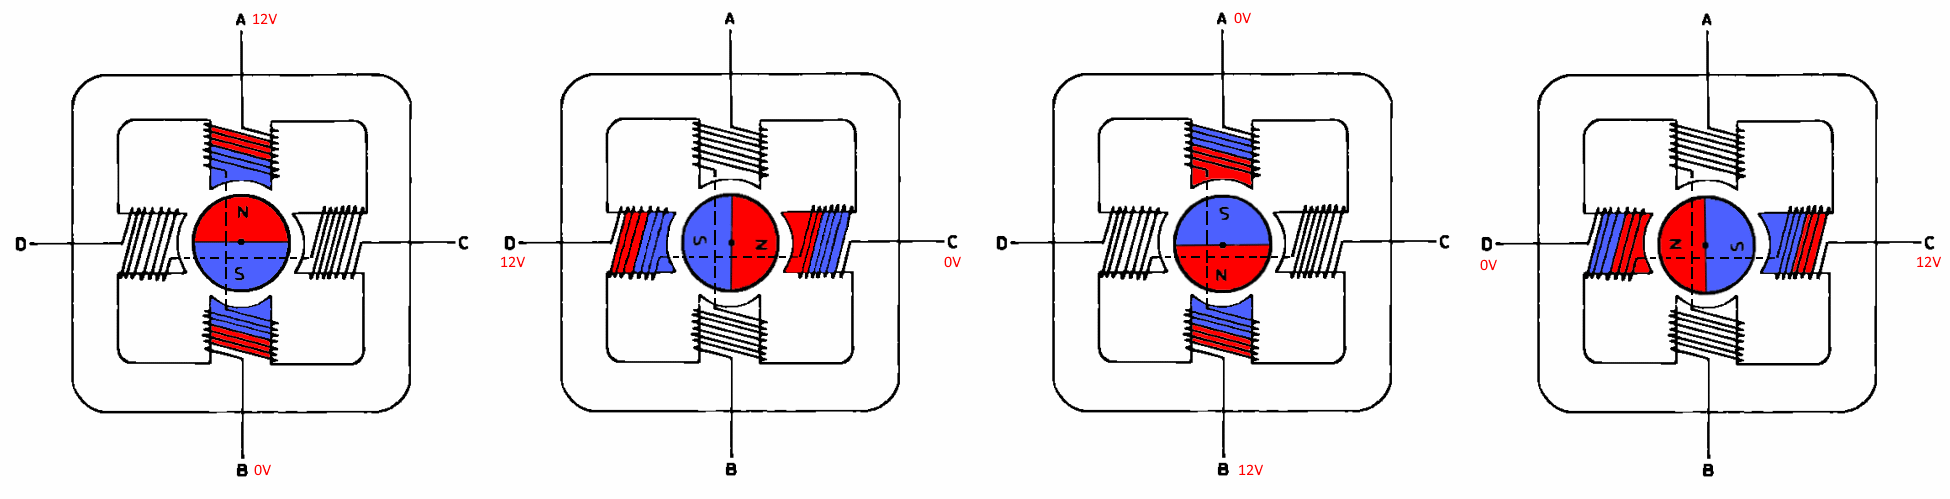
\includegraphics[scale=0.28]{../pictures/motor_min.png}
 \caption{Fonctionnement à pas complet avec un couple minimal\protect\footnotemark}
 \label{Motor_min}
\end{figure}
\footnotetext{Une animation du pas complet avec couple minimal est disponible sur \url{www.github.com/alphter/Sudoku-Plotter/blob/master/pictures/motor_min1.gif}}

\begin{figure}[!h]
 \center
 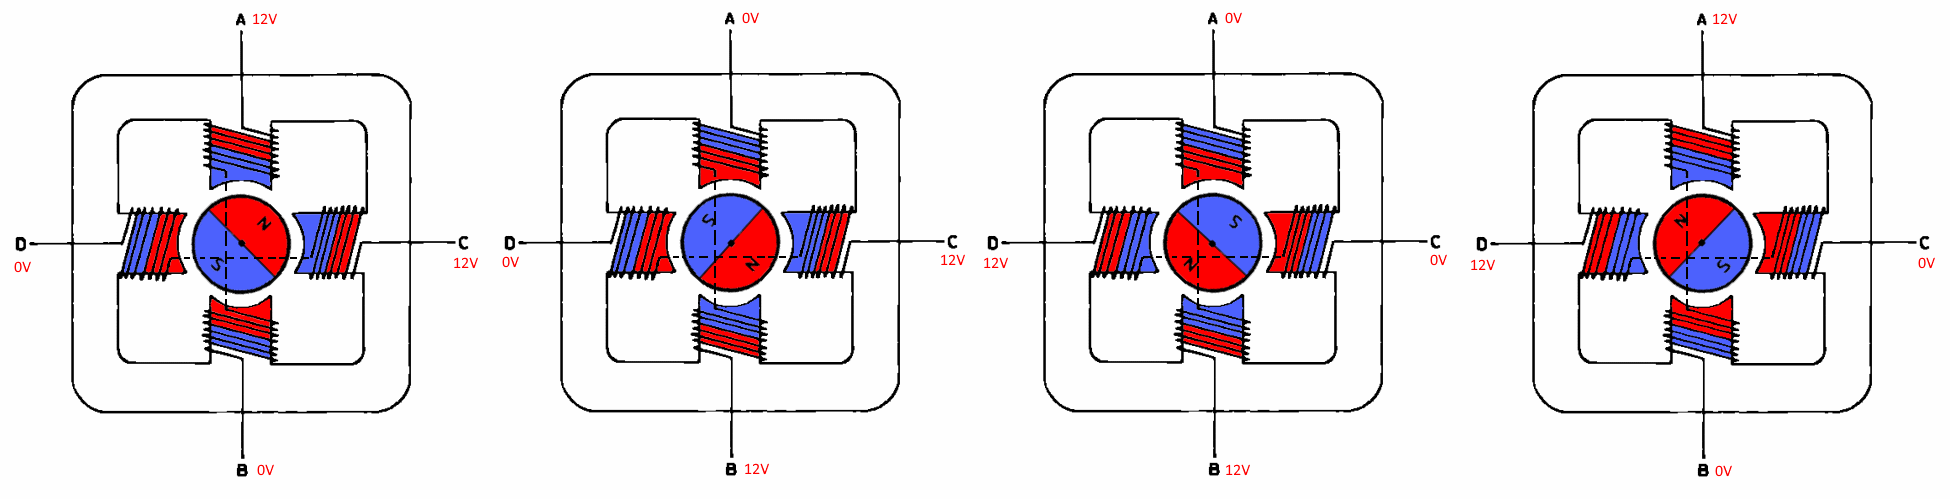
\includegraphics[scale=0.28]{../pictures/motor_max.png}
 \caption{Fonctionnement à pas complet avec un couple maximal\protect\footnotemark}
 \label{Motor_max}
\end{figure}
\end{center}
\footnotetext{Une animation du pas complet avec couple maximal est disponible sur \url{www.github.com/alphter/Sudoku-Plotter/blob/master/pictures/motor_max1.gif}}

Une autre différence entre l'alimentation d'une ou deux bobines réside également dans la position de l'axe des deux moteurs, la position de celui-ci est décalé d'un demi-pas. Le fonctionnement en demi-pas se base ainsi sur la combinaison de ces deux méthodes, ce qui entraîne un couple variable mais permet des déplacements plus précis.

\section{Drivers L293D}
Pour piloter les moteurs, nous utilisons des drivers L293D. Ces drivers présentent les avantages suivants :
\begin{itemize}[label=--,itemsep=0pt,font=\bf\Large,labelsep=5mm]
\item ils permettent l'utilisation d'une source de tension externe, la Raspberry ne pouvant fournir que du 5V;
\item ils intègrent deux ponts en H permettant d'inverser le courant circulant dans les bobines;
\item ils permettent d'éviter la création de courants induits dans la Raspberry, du faits des bobines, pouvant potentiellement l'endommager ou la détruire.
\end{itemize}

\begin{figure}[!h]
 \center
 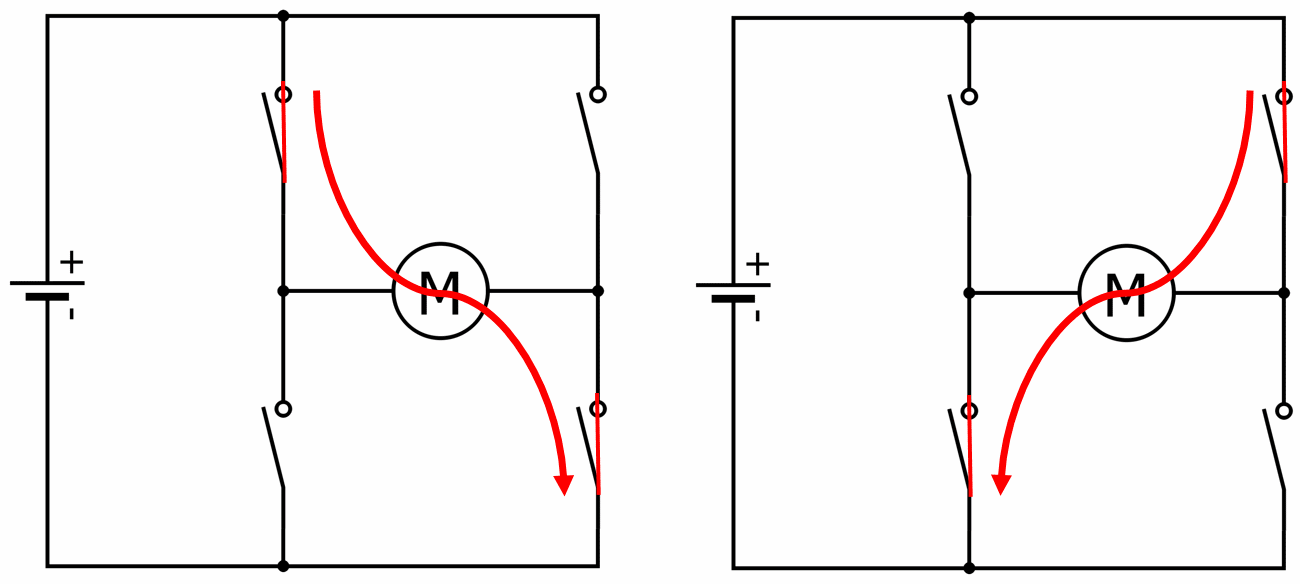
\includegraphics[scale=0.35]{../pictures/pontH.png}
 \caption{Utilité du pont en H, réalisé avec \emph{QElectroTech}}
 \label{pontH}
\end{figure}

Les ponts en H permettent l'alimentation d'une bobine dans les deux sens, ils permettent également de freiner le moteur en le court-circuitant. Celui-ci est constitué de quatre interrupteurs, conformément à la figure \ref{pontH}. Le moteur M représente une bobine. Les ponts en H sont utilisés dans quasiment tous les drivers des moteurs, que ce soit des moteurs continus ou des pas-à-pas. Les interrupteurs sont alors remplacés par des transistors, ce qui permet de les commander par une autre source d'alimentation (par exemple du 5V). Pour éviter la création de courants induits dans les bobines, on place généralement des diodes en parallèle des transistors (ou des interrupteurs). 

\begin{figure}[!h]
 \center
 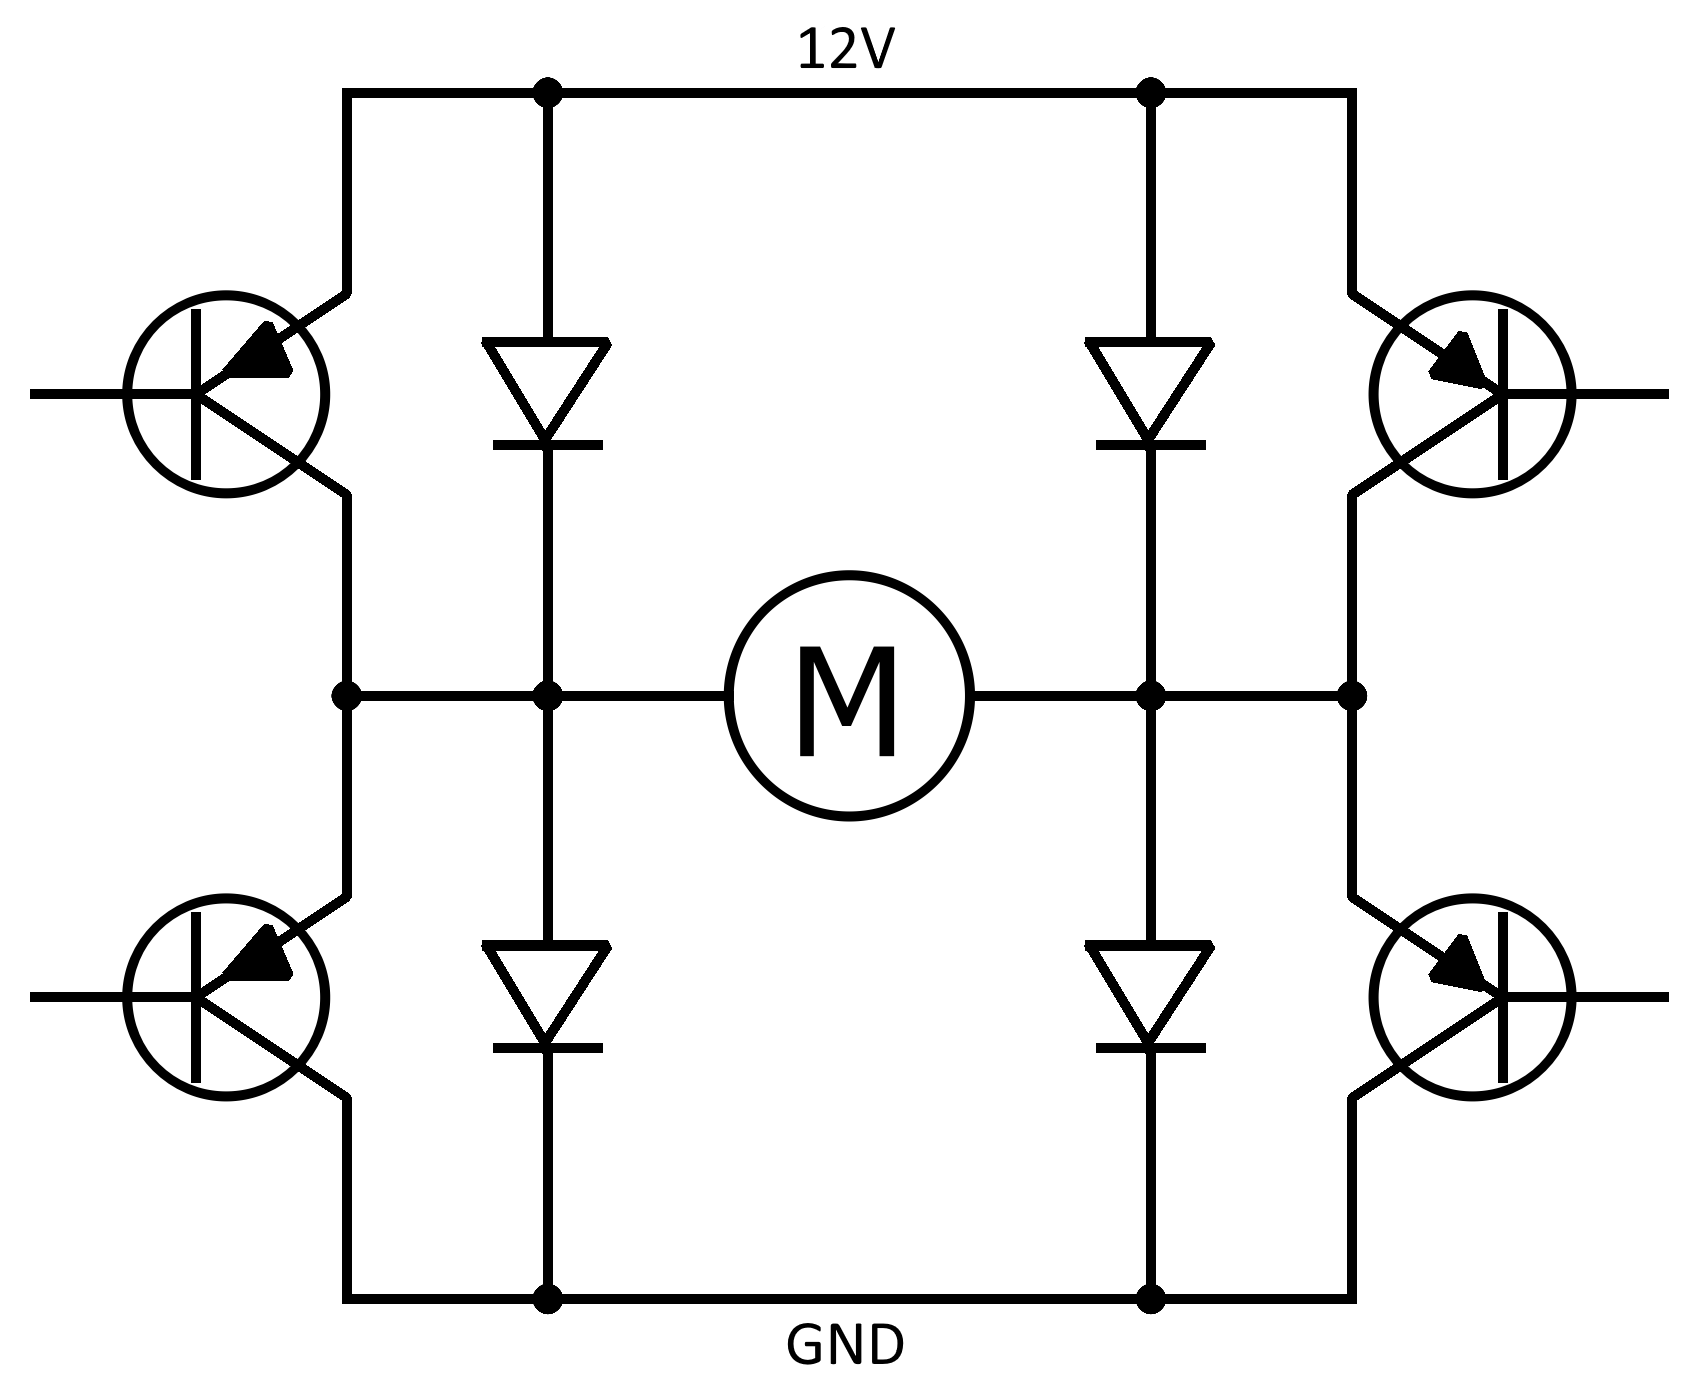
\includegraphics[scale=0.2]{../pictures/pont_en_H.png}
 \caption{Pont en H intégré dans les drivers, réalisé avec \emph{QElectroTech}}
 \label{pontH}
\end{figure}

Le driver L293D présente l'avantage d'intégrer deux pont en H ainsi que les diodes en parallèle ce qui permet des branchements aisés, sans besoin d'ajout d'autres composants. Comme nos moteurs intègrent deux bobines chacun, nous avons eu besoin de deux L293D, un par moteur.

\section{Schéma électrique}
Le schéma ci-joint représente les principales connections au sein de notre montage, même s'il ne présente ni l'écran LCD, ni le détail de l'alimentation de la \emph{Raspberry Pi} (notamment du convertisseur de tension).

Les moteurs deux bobines de chaque moteur sont reliées aux deux drivers l293D . Ceux-ci sont pilotés par quatre sorties GPIO qui envoient des impulsions au driver qui alimente les bobines en 12V à tour de rôle, ce qui permet à la fois de contrôler le sens et la vitesse de de rotation des moteurs, en choisissant à quelle fréquence envoyer les impulsions. La figure \ref{schema_elec} souligne la présence de deux alimentations différentes, à la fois l'alimentation 5V pour la \emph{Raspberry Pi} et l'alimentation 9V(ou 12V) pour alimenter les moteurs.
\begin{figure}[!h]
 \center
 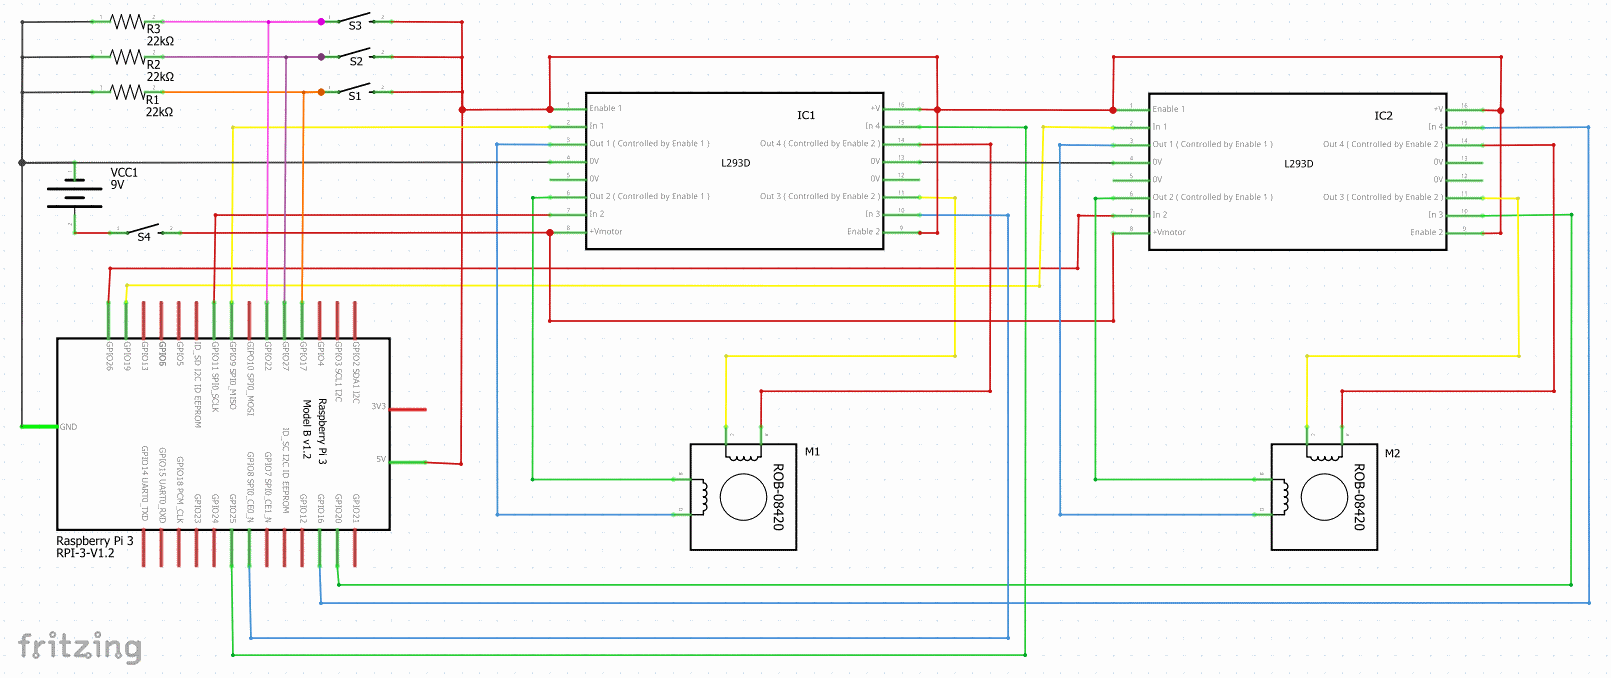
\includegraphics[scale=0.33]{../pictures/Sudoku_schema_electrique.png}
 \caption{Schéma électrique réalisé avec \emph{Fritzing}}
 \label{schema_elec}
\end{figure}

\newpage
\section{Premiers montages}
Nous avons réalisés nos premiers montages avec une breadboard facilitant les tests. Une simulation du schéma a également été réalisée sous \emph{Fritzing} :

\begin{figure}[!h]
 \center
 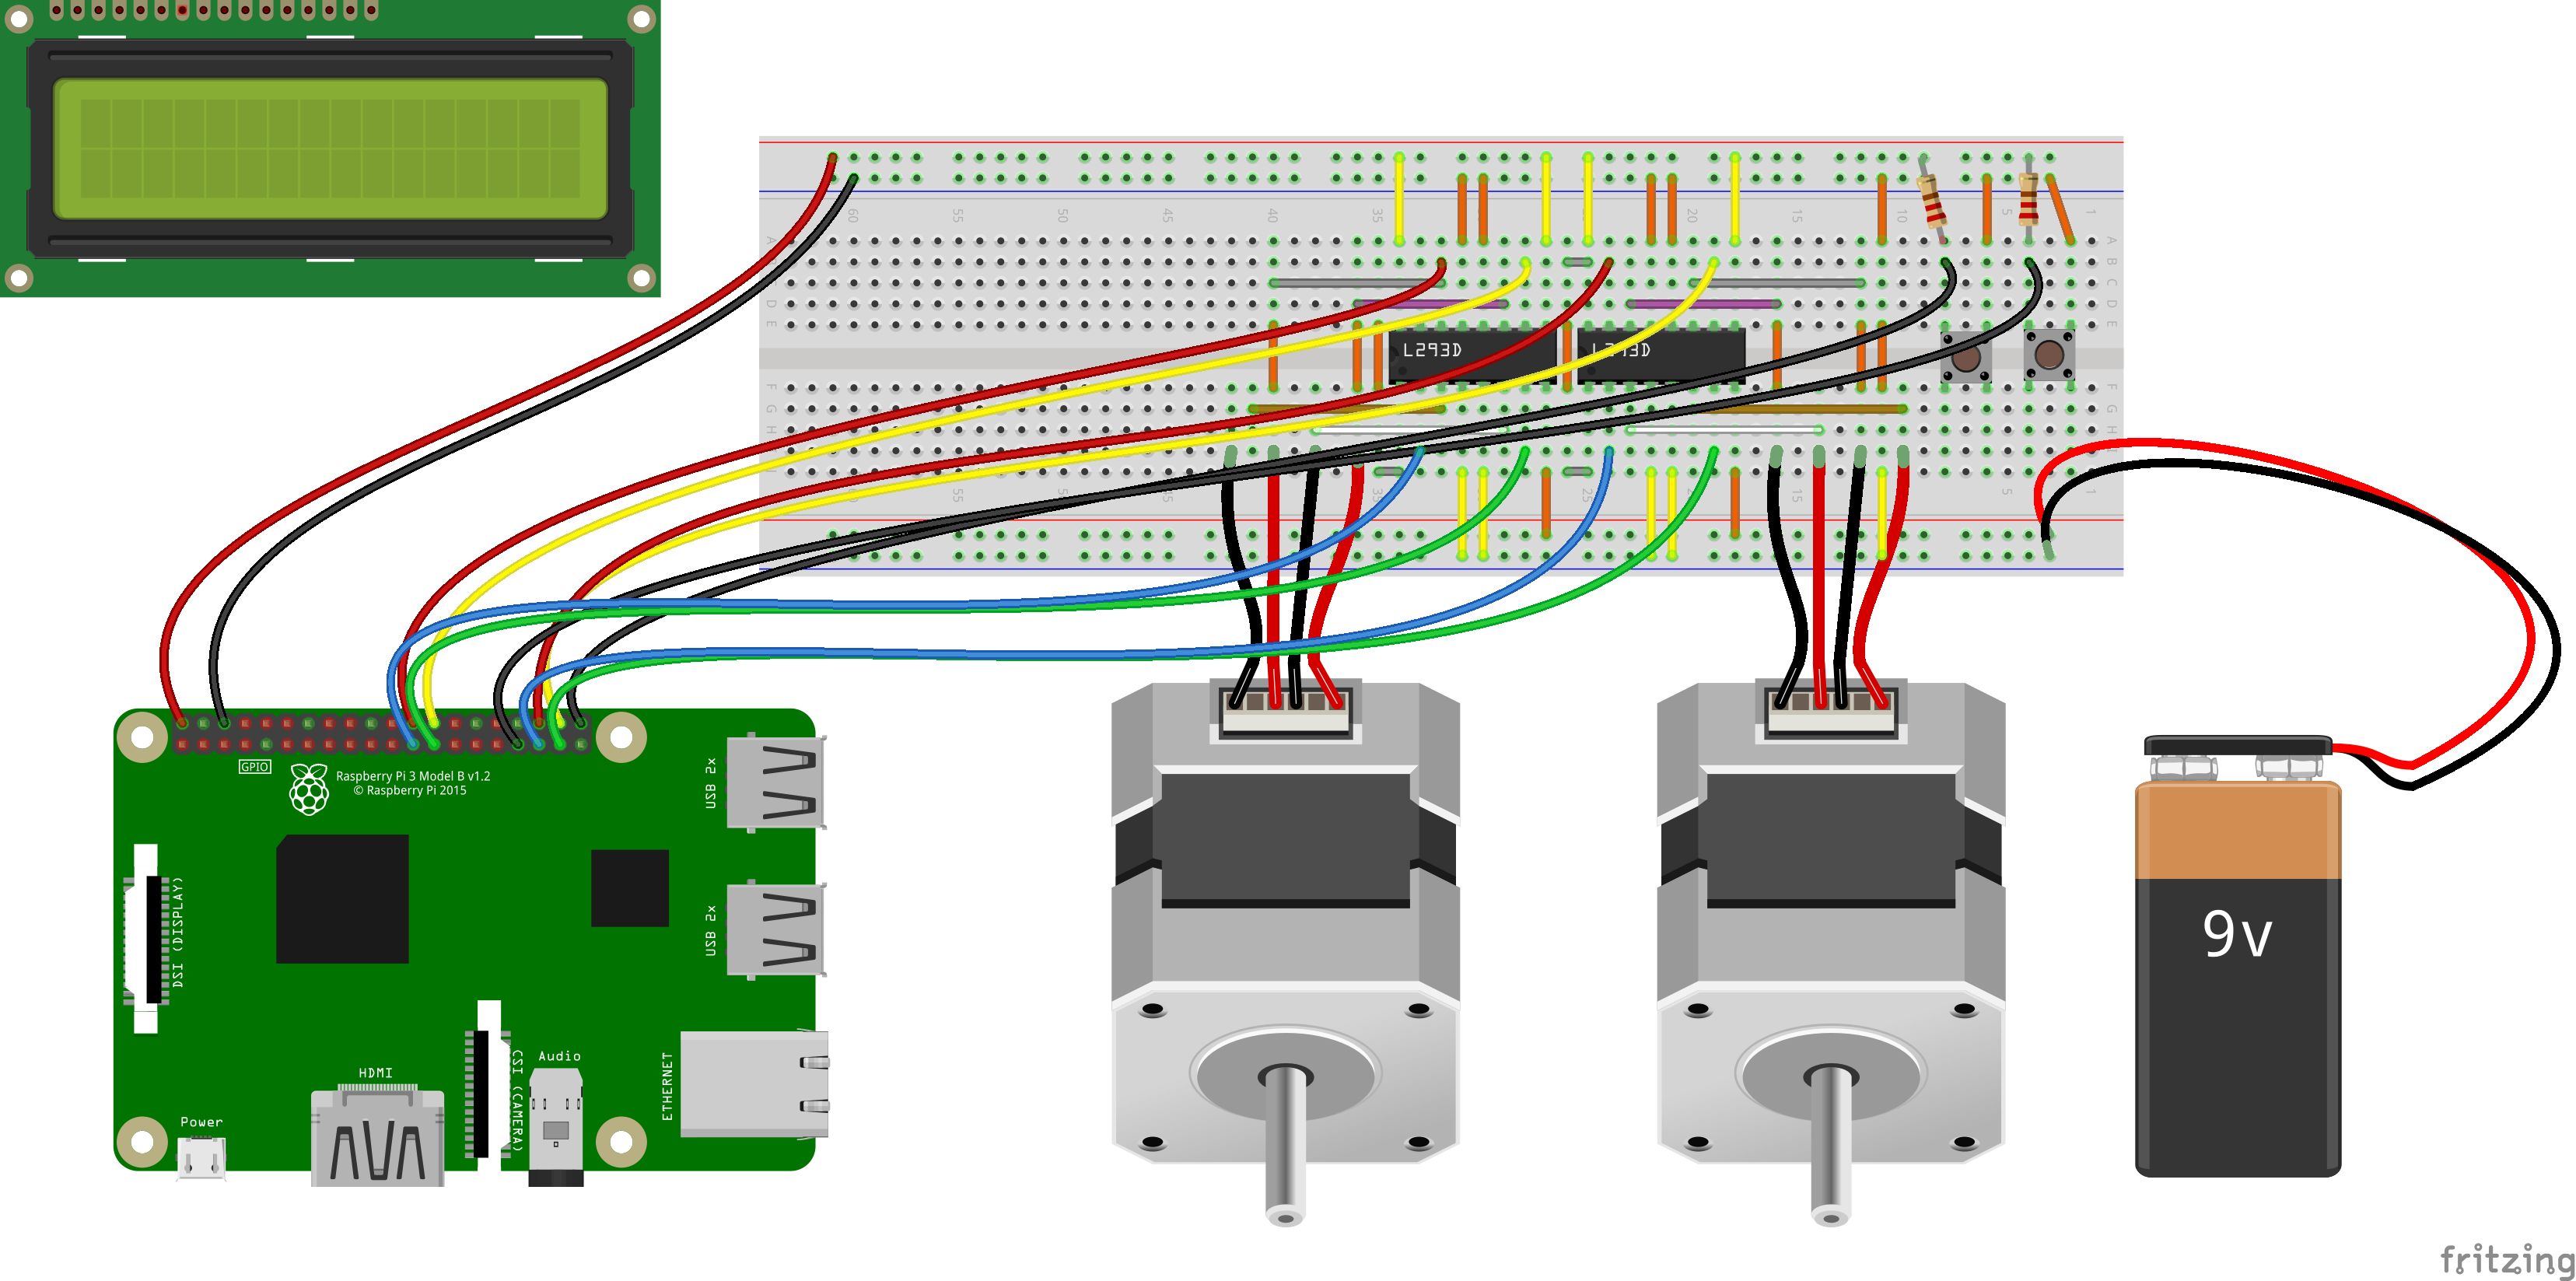
\includegraphics[scale=0.45]{../pictures/Sudoku_schema}
 \caption{Premier montage réalisé avec \emph{Fritzing}}
\end{figure}

\section{Circuit imprimé}
Pour rendre notre bras mécanique plus compact et ainsi rentrer dans le cadre de l'optimalité, nous avons souhaité remplacé la breadboard par une solution bien plus compacte, à savoir un circuit imprimé. Celui-ci sera enficher directement sur les ports GPIO de la Raspberry Pi. Nous avons de nouveau utilisé pour le réaliser le logiciel \emph{Fritzing}, permettant la réalisation du circuit sur deux couches (symbolisées par les couleurs orange et jaune), permettant un cablage plus facile, car permettant les croisements. Nous avons utilisé \emph{Fritzing} car il été assez facile de faire faire fabriquer le circuit imprimé pour une dizaine d'euros. Nous avions hésité à réaliser entièrement ce circuit par nous même, mais du fait de la présence de deux couches, cela se serait révéler très difficile et aurait sans doute coûté plus cher.

\begin{figure}[!h]
 \center
 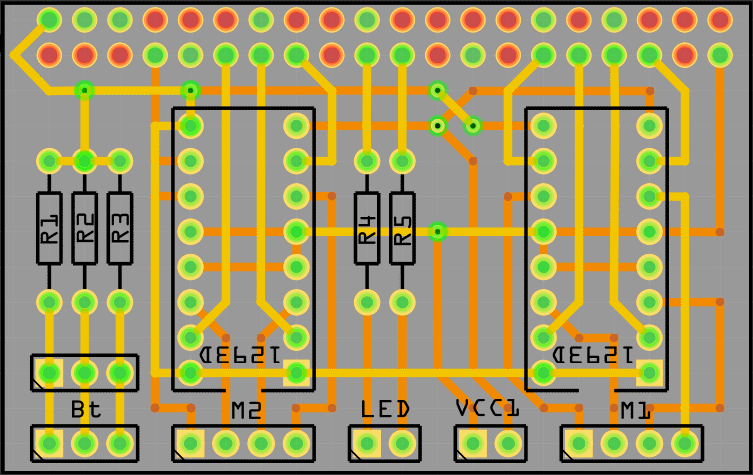
\includegraphics[scale=0.5]{../pictures/Sudoku_circuit_imprime.png}
 \caption{Circuit imprimé réalisé avec \emph{Fritzing}}
\end{figure}

\section{Écran LCD}
Pour rendre le bras mécanique autonome, nous avons intégré un écran LCD permettant à l'utilisateur de se repérer dans l'évolution des différents scripts sans disposer nécessairement d'un ordinateur ou d'un écran à proximité, ce qui permettait de rendre le bras plus autonome et plus facile d'utilisation. L'écran utilisé est un écran LCD 2x16.
\begin{figure}[!h]
 \center
 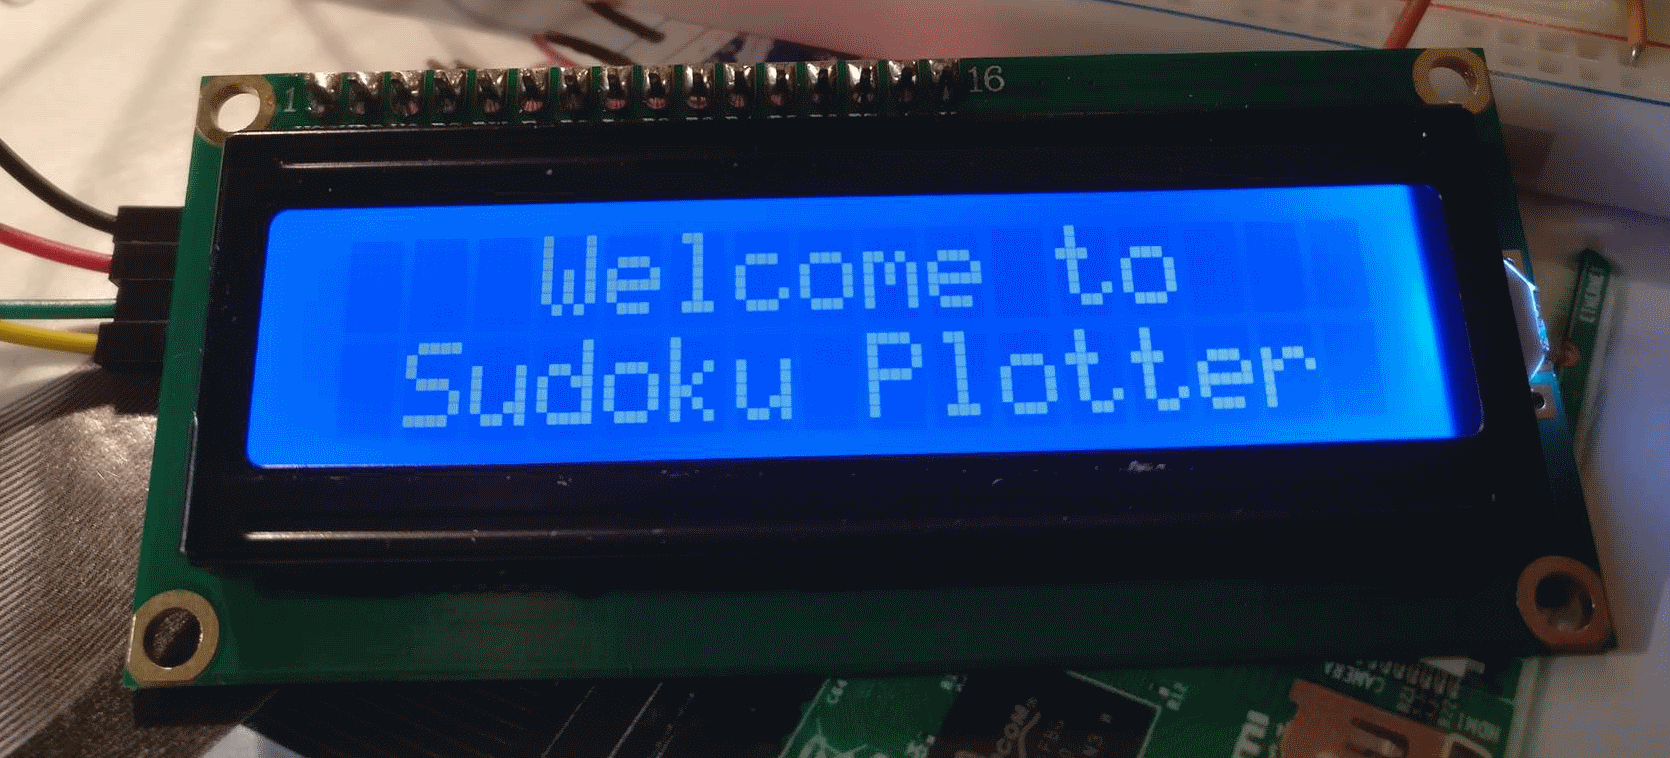
\includegraphics[scale=0.3]{../pictures/ecran_lcd}
 \caption{\'{E}cran LCD affichant le message de bienvenue}
\end{figure}


	\chapter{Informatique}
\section{Présentation globale}
	Tous les algorithmes développés dans le cadre de ce projet sont disponibles en annexe. Ils ont été, pour la plupart, développés sous Python 3, les autres sous Python 2 car certaines bibliothèques dont nous avions besoin, notamment pour la reconnaissance, n'était disponible que sous Python 2. 
	
	Nous avons développé une programmation modulaire, permettant de travailler simultanément sur le projet, sans pour autant poser de problème de logistique. Ainsi nous avons dissocié tous les scripts ; que ce soit la reconnaissance, la résolution, l'affichage, la gestion de la caméra ou des servo-moteurs, etc. Pour cela, nous avons développé une relation qualifiable de maître-esclave entre nos scripts. Chacun des scripts dépend d'un fichier principal, appelé \emph{main}, qui récupère les informations des autres scripts et donne les ordres adéquats à ceux-ci, selon la situation. Ainsi, les scripts ne sont pas reliés les uns aux autres mais seulement à ce script principal, ce qui permet d'ajouter ou d'enlever très facilement tel ou tel script, sans pour autant altérer le fonctionnement de l'ensemble, permettant ainsi de tester chacun des scripts très facilement.
	
	Il nous apparaissait de plus nécessaire de développer une programmation permettant l'exécution simultanée de plusieurs instructions, notamment pour les moteurs. En effet, les moteurs doivent absolument fonctionner de manière synchrone afin des déplacements les plus précis possibles. C'est pour cela que nous nous sommes basés sur ce qui pourrait être qualifiée de "programmation parallèle" qui permet l'exécution de plusieurs processus simultanément. Cela est rendu possible en Python par l'utilisation de la bibliothèque \emph{threading} depuis laquelle nous utilisons \emph{Thread} (signifiant \emph{processus} en français).
	
\newpage
\section{Reconnaissance du sudoku}
	Le script de reconnaissance du sudoku a été réalisé sous Python 2 avec le module de traitements d'image OpenCV. Il a été réalisé pour :
	\begin{itemize}[label=--]
	\item Reconnaître les chiffres dans une grille du sudoku
	\item Déterminer la position spatiale de la grille
	\end{itemize}
	On photographie la grille avec une caméra Raspberry Pi (V2) comme celle-ci :
\begin{figure}[!h]
 \center
 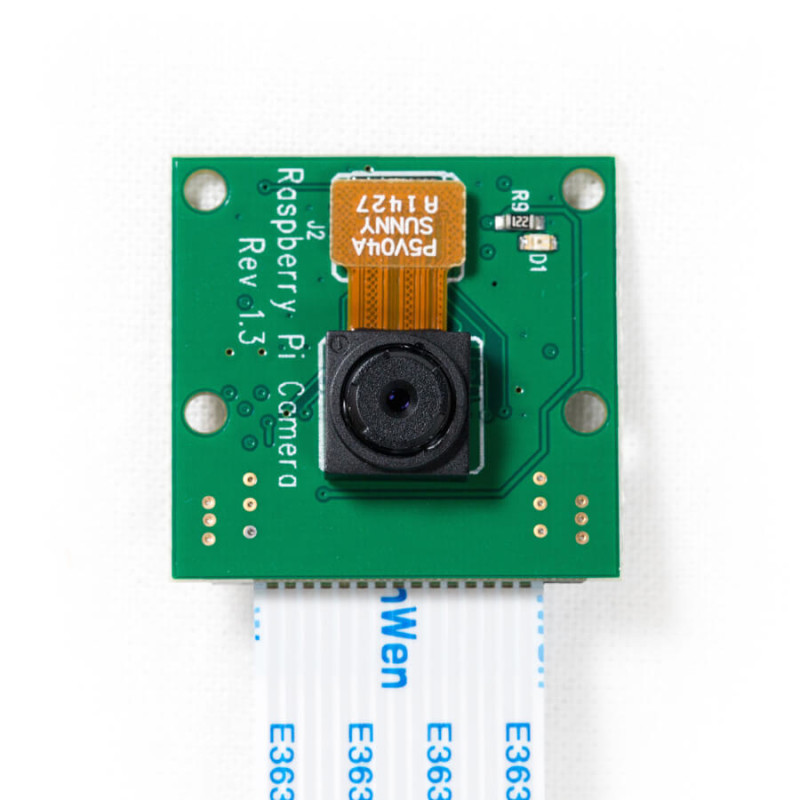
\includegraphics[scale=0.2]{../pictures/camera.jpg}
 \caption{Caméra Raspberry Pi V2}
\end{figure}

Voici la grille de sudoku qui nous servira d'exemple pour montrer toutes les actions du script :
\begin{figure}[!h]
 \center
 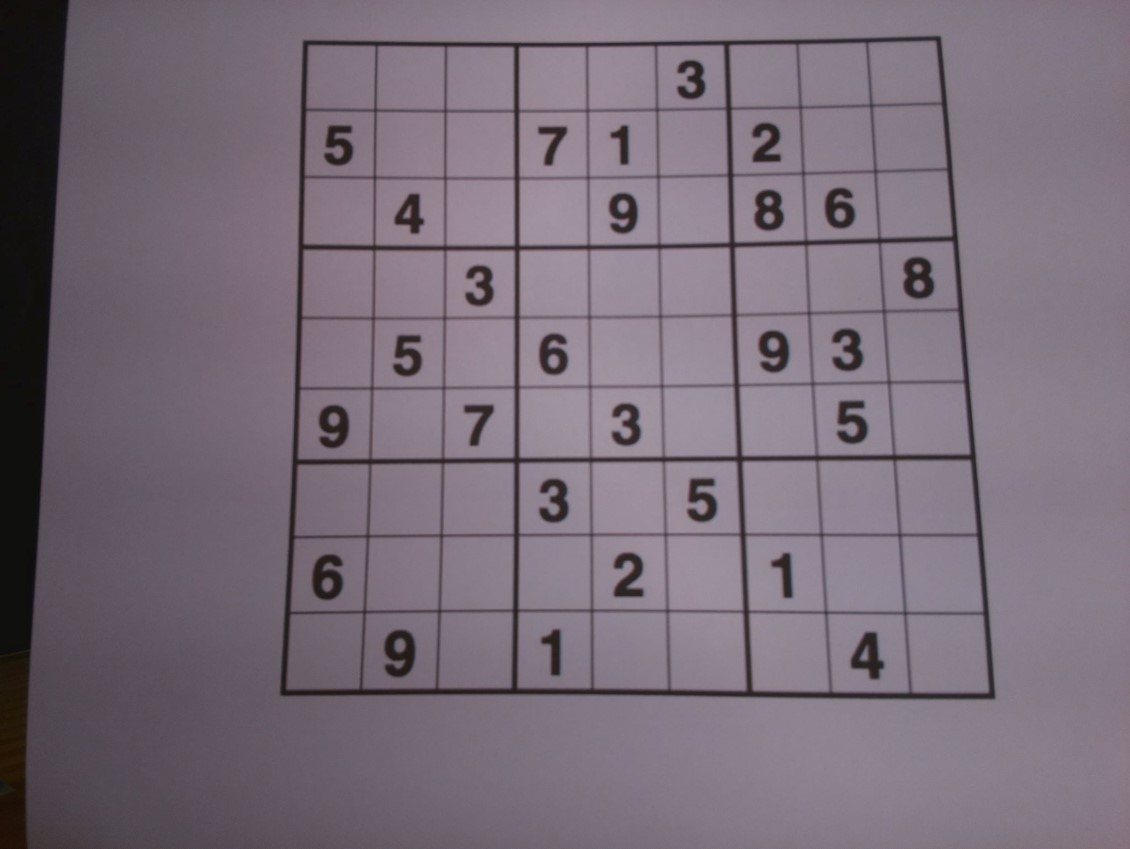
\includegraphics[scale=0.25]{../pictures/example.jpg}
 \caption{Exemple de grille de sudoku}
\end{figure}
\newpage
On applique sur cette photographie un filtre de type seuil (en anglais "threshold") qui va ensuite nous permettre de détecter les contours de la grille :

\begin{figure}[!h]
 \center
 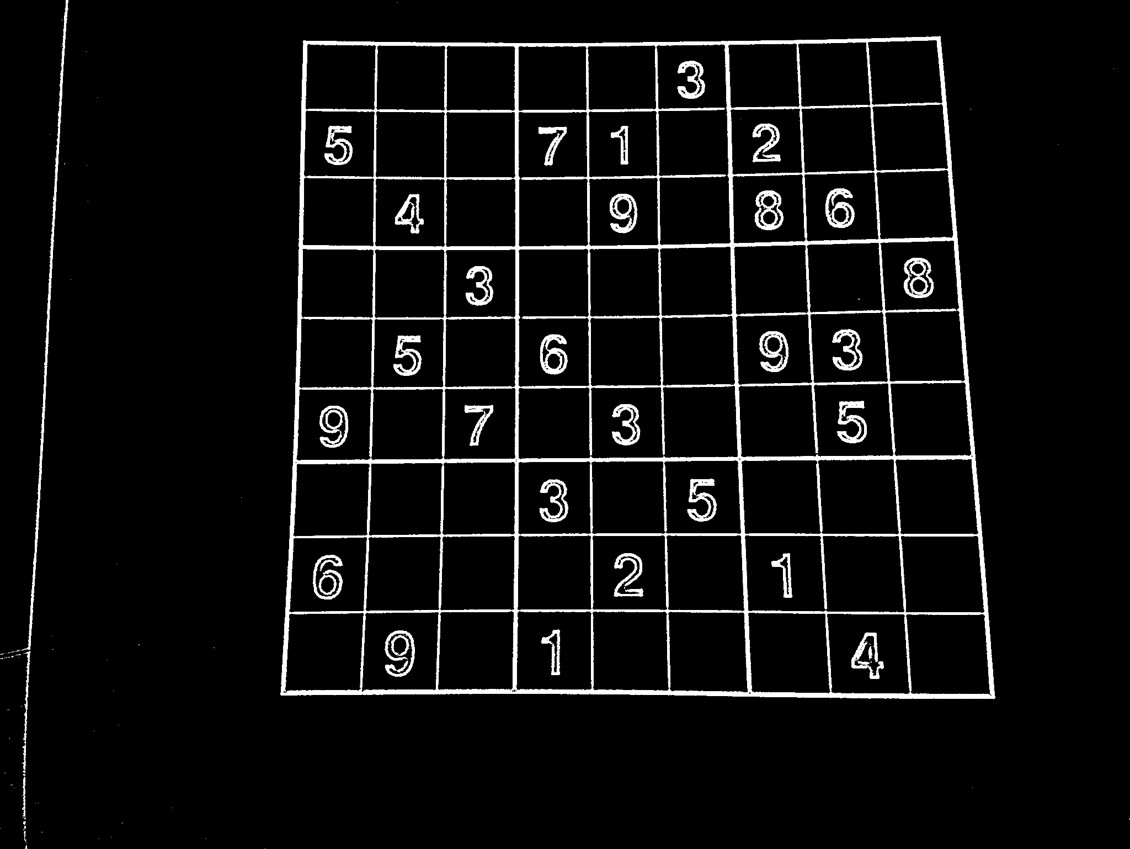
\includegraphics[scale=0.25]{../pictures/threshold.jpg}
 \caption{Exemple de grille "seuillée"}
 \end{figure}
 
Par cette transformation, on peut ensuite déterminer des équations de droites des contours extérieurs de la grille. Les coordonnées des intersections des droites seront celle des coins de la grille. \smallbreak On découpe alors la grille de la photographie initiale en supprimant les éventuels effets de perspective. 
 
\begin{figure}[!h]
 \center
 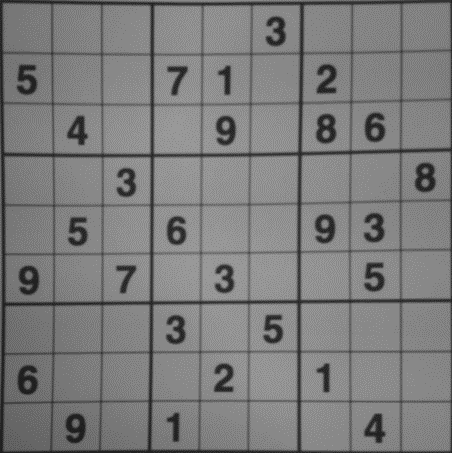
\includegraphics[scale=0.55]{../pictures/unperspectived.png}
 \caption{Exemple de grille découpée sans perspective}
\end{figure}
\newpage
On découpe chaque petite case de la grille comme ci-dessous :

\begin{figure}[!h]
 \center
 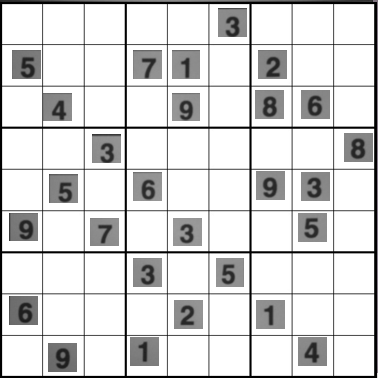
\includegraphics[scale=0.6]{../pictures/cutted.png}
 \caption{Exemple de grille où chaque chiffre a été découpé}
\end{figure}

On utilise ensuite un module de reconnaissance de digits pour détecter les chiffres et on obtient la grille suivante, prête à être résolue :

\begin{figure}[!h]
 \center
 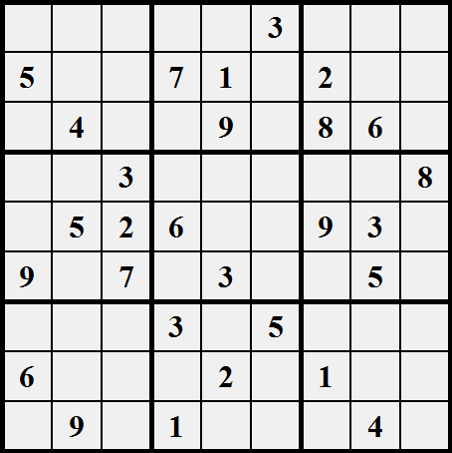
\includegraphics[scale=0.55]{../pictures/finished.png}
 \caption{Exemple de grille prête à être résolue}
\end{figure}

\newpage
\section{Résolution du sudoku}
\label{Resolution}
Pour résoudre une grille de sudoku, un joueur utilise différentes méthodes de résolution, qui sont purement algorithmiques. Il utilise en grande majorité deux méthodes qui peuvent permettre de résoudre une grande partie des grilles disponibles sur le marché. On appelle ces deux méthodes \emph{inclusion} et \emph{exclusion}. Cependant les grilles de niveau supérieur font appel à des méthodes plus subtiles et souvent plus difficiles à appliquer en pratique qui se basent généralement sur des \emph{paires} ou des \emph{triplets}. Les grilles les plus difficiles peuvent imposer au joueur de faire un choix entre plusieurs possibilités pour espérer mener à son terme la résolution. C'est sur ce constat que ce base la méthode dite de \emph{backtracking} (ou \emph{retour sur trace}), qui permet de résoudre toute grille de sudoku, même si celle-ci n'est pas valide et possède plusieurs solutions. Bien sûr cette liste n'est pas exhaustive et il existe d'autres méthodes de résolution, même si ces méthodes ne sont pas forcément très employés faciles d'emploi.

\paragraph{Inclusion: un seul candidat pour une case}
On dénombre pour chaque case vierge les chiffres pouvant être positionnés dans celle-ci. S'il n'y a qu'une seule possibilité alors elle est solution et est donc placée dans la case.
\begin{figure}[!h]
 \center
 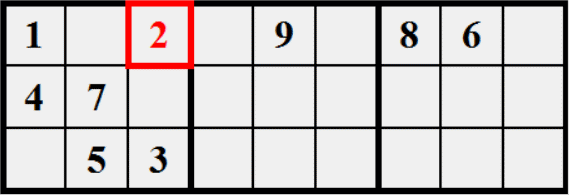
\includegraphics[scale=0.6]{../pictures/inclusion}
 \caption{Méthode d'inclusion pour une région}
\end{figure}

\paragraph{Exclusion: candidat unique pour une section}
Si pour un chiffre donné, on ne peut le placer dans une section que dans une seule case possible, alors ce chiffre est placé dans cette case
\begin{figure}[!h]
 \center
 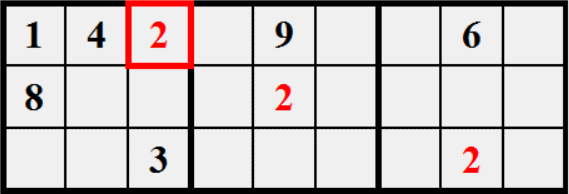
\includegraphics[scale=0.6]{../pictures/exclusion}
 \caption{Méthode d'exclusion pour une région}
\end{figure}

\paragraph{Paires} Si dans une section donnée, deux cases ne contiennent que deux \emph{candidats identiques}, alors ils ne peuvent être placés que dans ces deux cases, ce qui permet de les éliminer des autres possibilité pour la section
\begin{figure}[!h]
 \center
 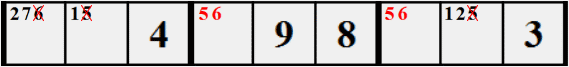
\includegraphics[scale=0.6]{../pictures/paire}
 \caption{Méthode des paires pour une ligne}
\end{figure}

La méthode des triplets est une généralisation de cette méthode à trois cases et non seulement deux.

\paragraph{Jumeaux} Si dans une section, un chiffre ne peut être placé que sur une ligne (resp. colonne), alors ce chiffre peut être supprimé des possibilités pour le reste de la ligne (resp.colonne). Cette méthode ne permet pas toujours de placer immédiatement celui-ci, mais permet de réduire les possibilités pour placer les autres.
\begin{figure}[!h]
 \center
 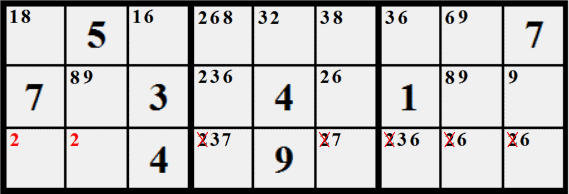
\includegraphics[scale=0.6]{../pictures/jumeaux}
 \caption{Méthode des jumeaux pour une ligne}
\end{figure}

\paragraph{Backtracking} Cette méthode\footnote{Une animation du \emph{backtracking} est disponible sur : \url{www.github.com/alphter/Sudoku-Plotter/blob/master/pictures/backtracking.gif}} consiste tout d'abord à lister pour chacune des cases vierges les chiffres qui pourraient correspondre. On part d'une case vierge quelconque qu'on remplit par un des chiffres pouvant théoriquement convenir, puis on liste les nouvelles possibilités des autres cases en fonction du chiffre précédemment ajouté puis on passe à la case suivante. S'il n'y a plus aucune possibilité, on revient sur nos pas et on change le chiffre qu'on venait d'ajouter en une autre possibilité. Si tout les chiffres possibles ont été testé, on revient de nouveau sur nos pas autant de fois que nécessaire, jusqu'à avoir compéter la totalité de la grille. 

Cette méthode ne peut pas être mise en oeuvre par un joueur, dans la mesure où elle lui demanderait énormément de temps, et ne présenterait pour lui aucun intérêt. Cependant, elle peut être indispensable pour les grilles diaboliques lorsque le joueur doit faire un choix, cette méthode est alors indispensable.
Pour une ordinateur également, cette méthode peut se révéler fastidieuse dans le cas où la solution n'apparait que très tardivement, et après beaucoup d'itérations. Elle est surtout efficace dans le cas général, mais peut être mise en défaut.

%\begin{center}
%	\animategraphics[width=0.6\linewidth]{24}{../pictures/backtracking/backtracking-}{1}{1001}
%\end{center}

\paragraph{} Partant de ce constat, nous avons tout d'abord implémenté la méthode de \emph{backtracking}, ainsi, il nous était possible de résoudre toutes les grilles possibles. \`{A} l'origine, notre algorithme parcourait la grille dans un ordre prédéfini, à savoir de haut en bas et de gauche à droite. Cependant, il pouvait arriver que pour certaines grilles, ce système n'était pas tout à fait optimale. C'est pourquoi, nous l'avons changé de sorte que l'algorithme commence par les cases présentant le moins de possibilités, permettant dans le cas général de diminuer le temps de résolution. Cependant, dans le pire des cas, cette solution ne présentait aucune différence en terme de temps de calculs. 

\paragraph{Temps de calculs} Au niveau informatique, ces méthodes ne se valent pas dans la mesure où elles sont plus ou moins fiables, efficaces et rapides. L'\emph{inclusion} et l'\emph{exclusion} sont comparables : elles sont rapides et efficaces mais ne permettent pas la résolution complète dans un certain nombre de cas. L'utilisation du \emph{backtracking} se révèle alors efficace en complément des deux précédentes, puisque cette méthode permet toujours de conclure. Les temps de calculs sont comparables pour toutes ces méthodes et sont de l'ordre du centième de secondes\footnote{Les résultats peuvent varier d'un machine à l'autre comme nous avons pu le constater, il est donc surtout intéressant de noter les différences d'ordres de grandeurs entre les différents résultats.}. La résolution peut parfois prendre plus d'une seconde mais cette situation ne s'est présentée que très rarement. Cependant, il peut arriver que pour des grilles très particulières, conçues pour tester la rapidité du \emph{backtracking}, la résolution du sudoku prenne bien plus de temps, jusqu'à 30 secondes. En utilisant les trois méthodes de manière couplée, le temps de calculs diminue pour arriver à seulement 20 secondes. Une utilisation couplée des méthodes est bien plus efficace car permet d'éliminer immédiatement toutes les possibilités évidentes, indétectables en \emph{backtracking}, pour ensuite l'utiliser éventuellement si la grille n'est pas résolue.


\section{Interface graphique}
Pour rendre la résolution plus simple d'utilisation, nous avons décidé d'ajouter une interface graphique. Le cahier des charges qu'elle devait vérifier était assez stricte. Elle devait pouvoir afficher, avant toute chose, une grille de sudoku qui devait dès lors être facilement modifiable. Pour cela, nous avons donc créé différents menus ; l'un permettant donc l'édition de la grille, un autre permettant de choisir la méthode de résolution, ainsi qu'un menu de résolution. 

\paragraph{Édition} Lors de l'édition de la grille, un carré rouge apparait, déplaçable avec les flèches directionnelles, il suffit alors pour modifier la case de rentrer un chiffre de 0 à 9, 0 correspondant à une case vierge. Il est également possible de sauvegarder une grille ou encore de récupérer une grille déjà enregistrée.

\begin{figure}[!h]
 \center
 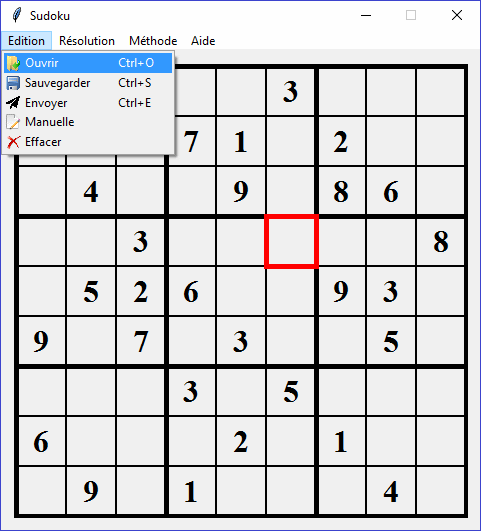
\includegraphics[scale=0.55]{../pictures/Sudoku_edition}
 \caption{Interface graphique affichant le menu Edition}
\end{figure}
\newpage
\paragraph{Résolution}Ce menu permet de lancer la résolution, et permet également de choisir entre une résolution rapide ou une résolution pas-à-pas permettant à l'utilisateur d'observer le fonctionnement de ces algorithmes.

\begin{figure}[!h]
 \center
 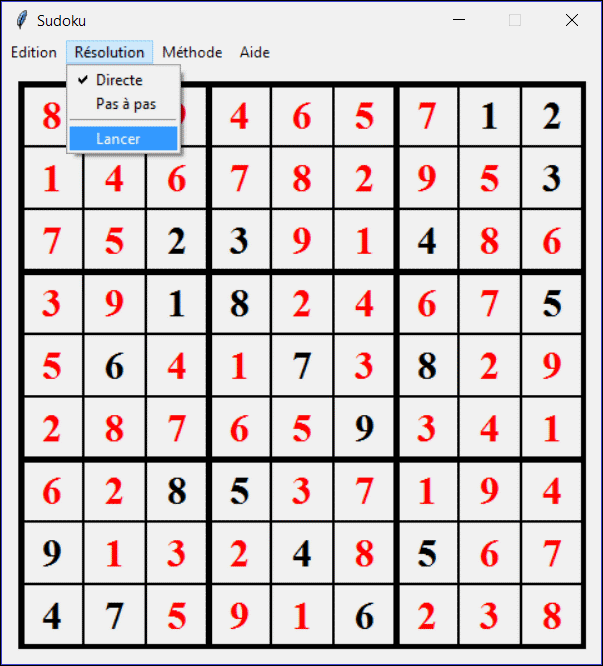
\includegraphics[scale=0.55]{../pictures/Sudoku_resolution}
 \caption{Interface graphique affichant le menu Édition}
\end{figure}

\paragraph{Méthode}Le choix de la méthode se fait avec le menu \emph{Méthode}, qui permet de choisir la méthode de résolution parmi l'\emph{inclusion}, l'\emph{exclusion} et le \emph{backtracking} ou de choisir une méthode dite \emph{globale}, s'appuyant sur tous les algorithmes, permettant ainsi d'être la plus rapide possible.

\section{Contrôle des moteurs et écriture}
\subsection*{Moteurs pas-à-pas}
Les moteurs se devaient de fonctionner simultanément pour des questions de précision évidentes. Comme nous l'avons dit précédemment \footnote{cf section \ref{Elec_stepper} à la page \pageref{Elec_stepper}}, il suffit d'envoyer des impulsions dans les bobines à la bonne fréquence pour faire tourner les moteurs à la bonne vitesse et dans le bon sens. Ces impulsions sont envoyés au deux moteurs de manière cycliques, un cycle étant constitué de quatre séquences. 

\subsection*{Coordonnées polaires}
Par soucis de compacité et ainsi s'inscrire dans l'optimalité du programme, nous avons décidé de développer une structure se basant sur les coordonnées polaires, permettant des dimensions maximum de 40 par 10 cm. L'utilisation de telles coordonnées nécessitait une plus grande précision et relevait donc d'un plus grand défi technique. Les coordonnées polaires ne sont de plus, que très peu utilisés pour ce type de système, ce qui nous à incité à développer une structure se basant sur ces coordonnées.
\begin{figure}[!h]
 \center
 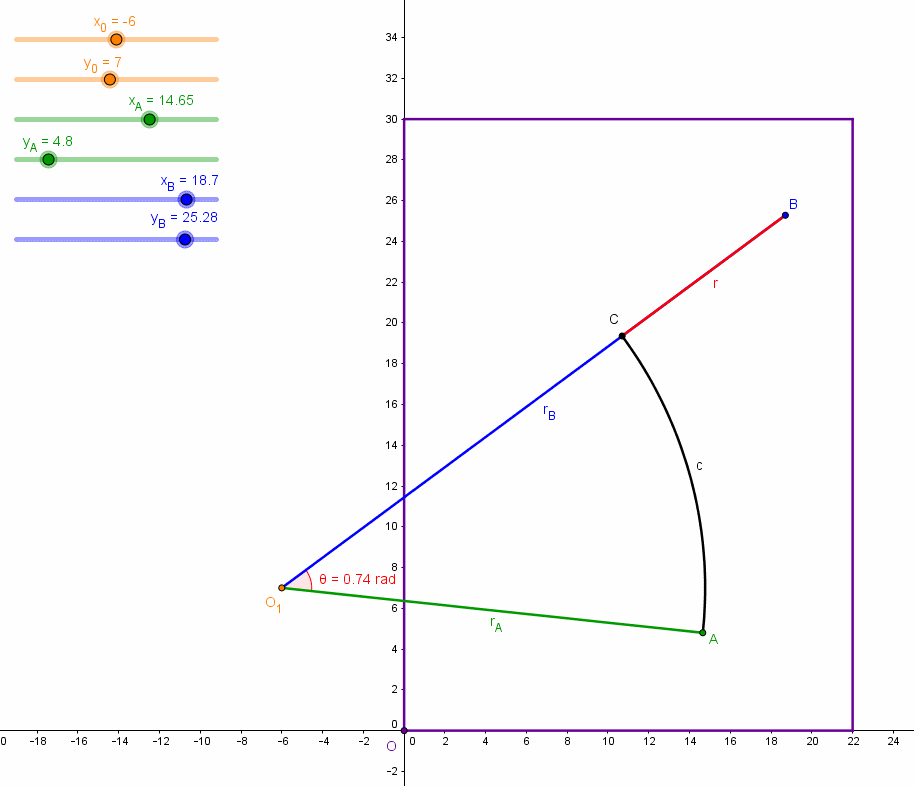
\includegraphics[scale=0.5]{../pictures/Changement_repere}
 \caption{Changement de repères réalisé avec \emph{Geogebra}}
\end{figure}

\subsection*{Écriture des digits}
Nous souhaitions dès le début pouvoir écrire des grilles de différentes tailles, et non des grilles de tailles fixes. C'est pourquoi nous avons basé le script d'écriture sur du point par point, permettant de choisir la précision théorique des chiffres tracés. Cependant les moteurs pas-à-pas ne pouvant se déplacer que d'un pas fixé de 1.8\degre, une trop grande précision ne pourrait entraînerait que des déplacements nuls des moteurs, c'est pourquoi cette manière de programmation permet un compromis entre précision théorique et précision pratique.
\begin{figure}[!h]
 \center
 
\includegraphics[scale=0.35]{../pictures/numbers}
 \caption{Chiffres d'une précision théorique assez faible}
\end{figure}
\newpage
En augmentant la précision théorique, on obtient des chiffres quasiment continus permettant d'obtenir la figure suivante :

\begin{figure}[!h]
 \center
 \includegraphics[scale=0.45]{../pictures/Sudoku_points}
 \caption{Grille de sudoku en point par point tracée avec \emph{MatplotLib}}
\end{figure}

Il faut prévoir dans le script la possibilité d'envoyer une impulsion au servomoteur afin qu'il lève le stylo lorsqu'un chiffre a été tracée afin d'éviter que les chiffres ne soient reliés entre eux, comme le suggère la figure \ref{sudoku_trace}.

\begin{figure}[!h]
 \center
 \includegraphics[scale=0.45]{../pictures/Sudoku_relies}
 \caption{Grille de sudoku tracée avec \emph{MatplotLib}}
 \label{sudoku_trace}
\end{figure}

\chapter*{Conclusion}
\addcontentsline{toc}{chapter}{Conclusion}
Ce TIPE a été très bénéfique et nous a tout d'abord permis d'améliorer les compétences acquises l'an dernier en Python.

De plus, de nombreuses nouvelles compétences ont du être mises en œuvre :

\begin{itemize}[label=--]
\item le contrôle de moteurs à l'aide d'une Raspberry Pi
\item la conception de pièces en 3D

\end{itemize}
Tous les scripts et ce dossier sont disponibles sur GitHub\footnote{Sudoku Plotter - \url{www.github.com/alphter/Sudoku-Plotter/}}

\chapter*{Remerciements}
\addcontentsline{toc}{chapter}{Remerciements}

Nous remercions M. Couvez pour ses précieux conseils et Tristan Vajente pour les impressions de pièces en 3D.

%\printbibliography
\nocite{*}
\appendix

\begin{changemargin}{-2cm}{-4cm}

\addcontentsline{toc}{chapter}{Scripts Python}
\label{Scripts}
\chapter*{Script principal}
\label{main}
%\inputminted[fontsize=\scriptsize, linenos=true]{Python}{../script/main.py}

\chapter*{Script de résolution des sudokus}
\label{resolution}
%\inputminted[fontsize=\scriptsize, linenos=true]{Python}{../script/resolution.py}

\chapter*{Script de gestion de la caméra}
\label{camera}
%\inputminted[fontsize=\scriptsize, linenos=true]{Python}{../script/camera.py}

\chapter*{Script d'affichage du sudoku}
\label{display}
%\inputminted[fontsize=\scriptsize, linenos=true]{Python}{../script/display.py}

\chapter*{Script de gestion des moteurs pas-à-pas}
\label{step_motor}
%\inputminted[fontsize=\scriptsize, linenos=true]{Python}{../script/step_motor.py}

\chapter*{Script permettant l'écriture d'un sudoku}
\label{write}
%\inputminted[fontsize=\scriptsize, linenos=true]{Python}{../script/write.py}
\addcontentsline{toc}{chapter}{Mises en plan des pièces conçues en 3D}

\chapter*{Mise en plan du chariot}
\begin{figure}[!h]
 \center
 \includegraphics[scale=1]{../3Dmodels/chariot.png}
\end{figure}

\chapter*{Mise en plan du support du stylo}
\begin{figure}[!h]
 \center
 \includegraphics[scale=1]{../3Dmodels/supportstylo.png}
\end{figure}

\chapter*{Mise en plan du lien chariot/caméra}
\begin{figure}[!h]
 \center
 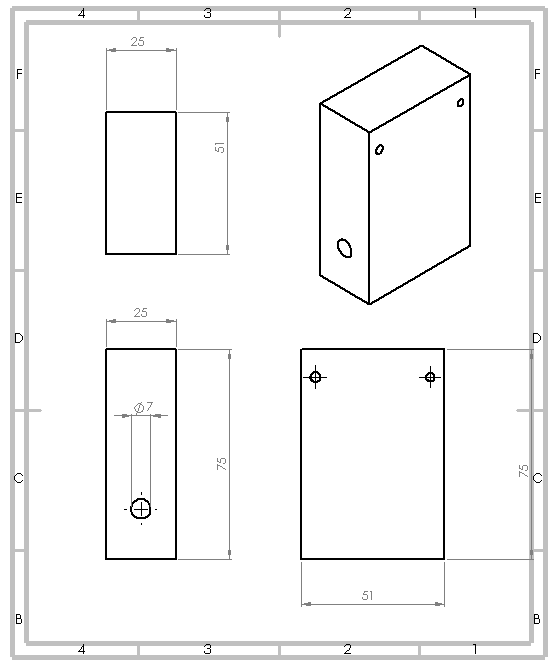
\includegraphics[scale=0.95]{../3Dmodels/camerachariot.png}
\end{figure}

\chapter*{Mise en plan du support de la caméra}
\begin{figure}[!h]
 \center
 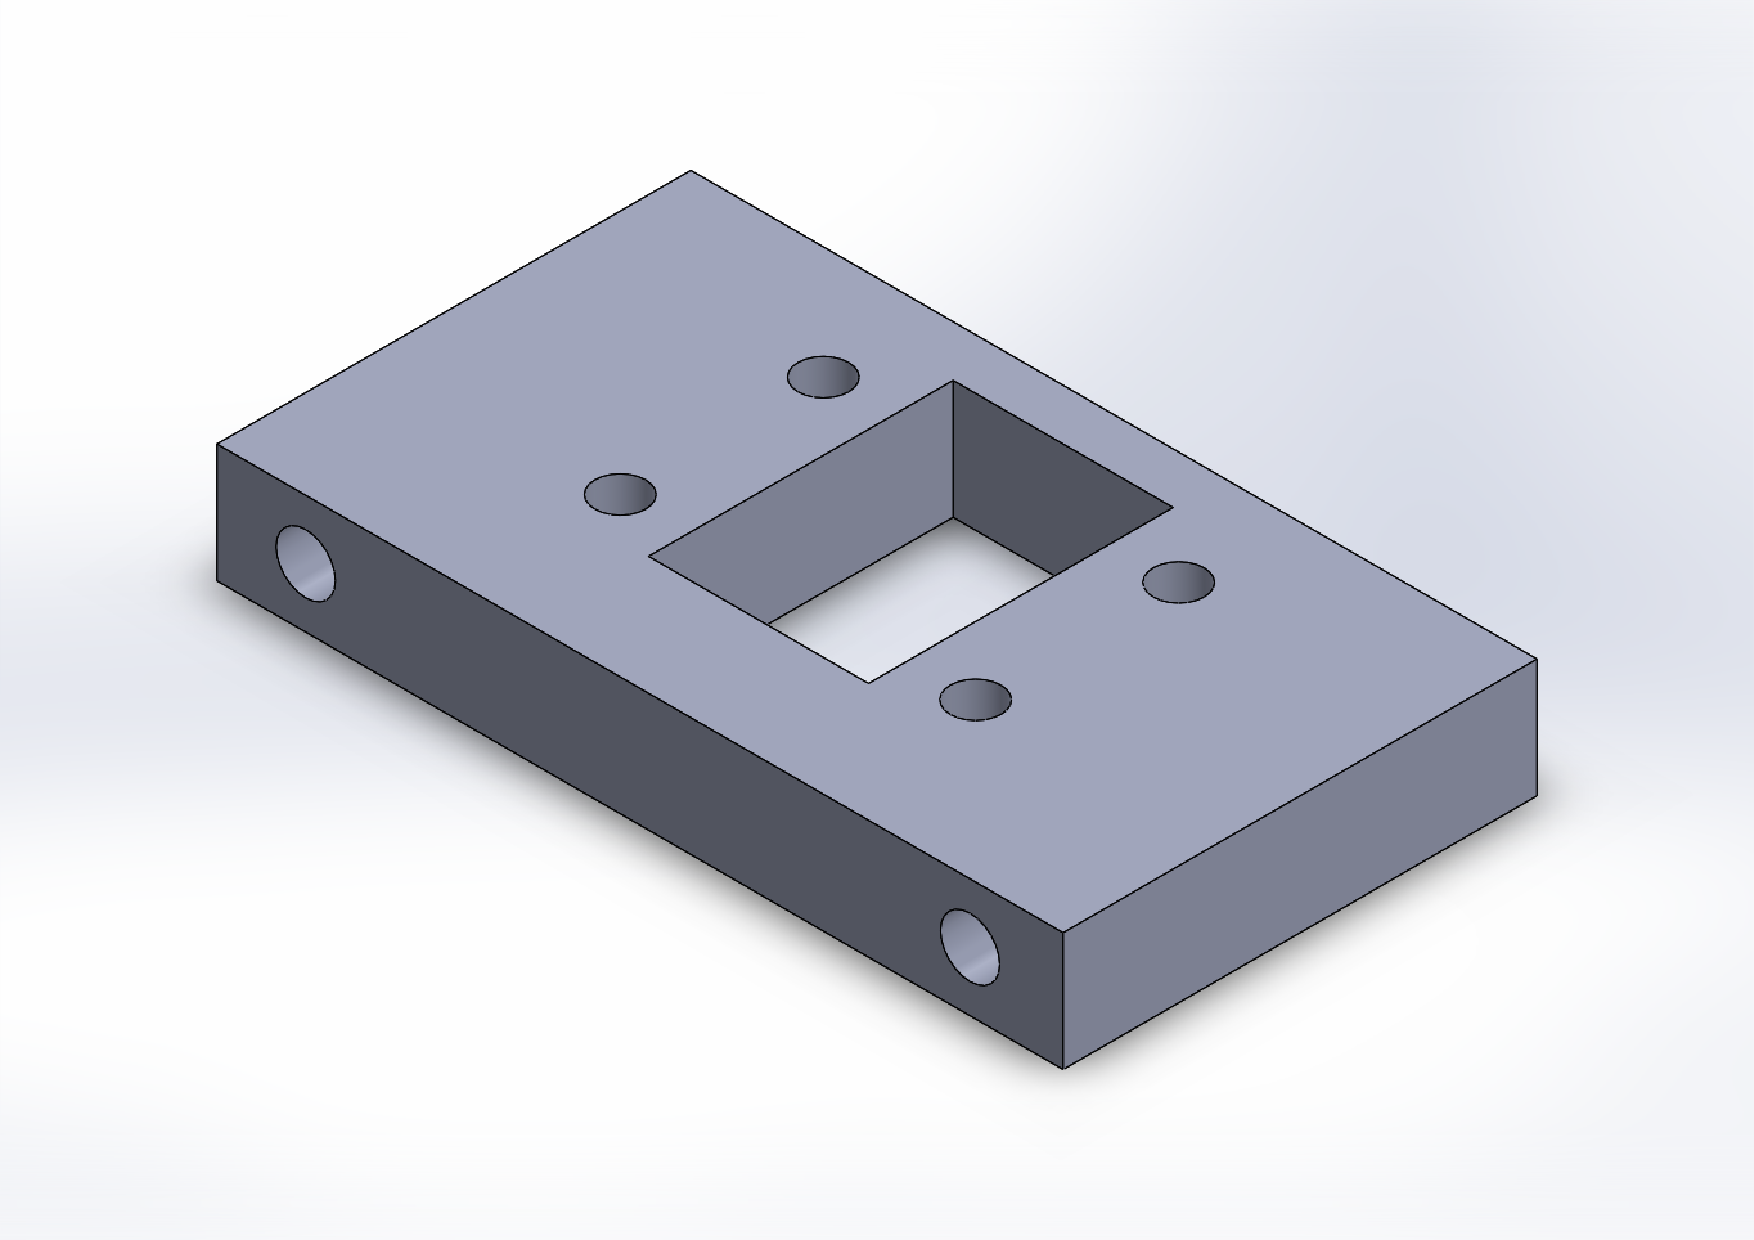
\includegraphics[scale=0.95]{../3Dmodels/camera.png}
\end{figure}

\end{changemargin}

\end{document}
